\documentclass[a5paper, 10pt]{article}

% Текст
\usepackage[utf8]{inputenc} % UTF-8 кодировка
\usepackage[russian]{babel} % Русский язык
\usepackage{indentfirst} % красная строка в первом параграфе в главе
% Отображение страниц
\usepackage{geometry} % размеры листа и отступов
\geometry{
	left=12mm,
	top=25mm,
	right=15mm,
	bottom=17mm,
	marginparsep=0mm,
	marginparwidth=0mm,
	headheight=10mm,
	headsep=7mm,
	nofoot}
\usepackage{afterpage,fancyhdr} % настройка колонтитулов
\pagestyle{fancy}
\fancypagestyle{style}{ % создание нового стиля style
	\fancyhf{} % очистка колонтитулов
	\fancyhead[LO, RE]{Лабораторная работа № 1 } % название документа наверху
	\fancyhead[RO, LE]{ Кодирование и шифрование} % название section наверху
	\fancyfoot[RO, LE]{\thepage} % номер страницы справа внизу на нечетных и слева внизу на четных
	\renewcommand{\headrulewidth}{0.25pt} % толщина линии сверху
	\renewcommand{\footrulewidth}{0pt} % толцина линии снизу
}
\fancypagestyle{plain}{ % создание нового стиля plain -- полностью пустого
	\fancyhf{}
	\renewcommand{\headrulewidth}{0pt}
}
\fancypagestyle{title}{ % создание нового стиля title -- для титульной страницы
	\fancyhf{}
	\fancyhead[C]{{\footnotesize
			Министерство образования и науки Российской Федерации\\
			Федеральное государственное автономное образовательное учреждение высшего образования
	}}
	\fancyfoot[C]{{\large 
			Санкт-Петербург, 2023-2024
	}}
	\renewcommand{\headrulewidth}{0pt}
}

% Математика
\usepackage{amsmath, amsfonts, amssymb, amsthm} % Набор пакетов для математических текстов
%\usepackage{dmvnbase} % мехматовский пакет latex-сокращений
\usepackage{cancel} % зачеркивание для сокращений
% Рисунки и фигуры
\usepackage[pdftex]{graphicx} % вставка рисунков
\usepackage{wrapfig, subcaption} % вставка фигур, обтекая текст
\usepackage{caption} % для настройки подписей
\captionsetup{figurewithin=none,labelsep=period, font={small,it}} % настройка подписей к рисункам
% Рисование
\usepackage{tikz} % рисование
\usepackage{circuitikz}
\usepackage{pgfplots} % графики
% Таблицы
\usepackage{multirow} % объединение строк
\usepackage{multicol} % объединение столбцов
% Остальное
\usepackage[unicode, pdftex]{hyperref} % гиперссылки
\usepackage{enumitem} % нормальное оформление списков
\setlist{itemsep=0.15cm,topsep=0.15cm,parsep=1pt} % настройки списков
% Теоремы, леммы, определения...
\theoremstyle{definition}
\newtheorem{Def}{Определение}
\newtheorem*{Axiom}{Аксиома}
\theoremstyle{plain}
\newtheorem{Th}{Теорема}
\newtheorem{Lem}{Лемма}
\newtheorem{Cor}{Следствие}
\newtheorem{Ex}{Пример}
\theoremstyle{remark}
\newtheorem*{Note}{Замечание}
\newtheorem*{Solution}{Решение}
\newtheorem*{Proof}{Доказательство}
% Свои команды
\newcommand{\comb}[1]{\left[\hspace{-4pt}\begin{array}{l}#1\end{array}\right.\hspace{-5pt} } % совокупность уравнений
% Титульный лист
\usepackage{csvsimple-l3}
\newcommand*{\titlePage}{
	\thispagestyle{title}
	\begingroup
	\begin{center}
		%		{\footnotesize
			%			Министерство образования и науки Российской Федерации\\
			%			Федеральное государственное автономное образовательное учреждение высшего образования
			%		}
		%		
		\vspace*{6ex}
		
		{\small
			САНКТ-ПЕТЕРБУРГСКИЙ НАЦИОНАЛЬНЫЙ ИССЛЕДОВАТЕЛЬСКИЙ УНИВЕРСИТЕТ ИТМО	
		}
		
		\vspace*{2ex}
		
		{\normalsize
			Факультет систем управления и робототехники
		}
		
		\vspace*{15ex}
		
		{\Large \bfseries 
			Лабораторная работа № 1
		}
\vspace*{2ex}
	{\Large \bfseries 
			
"Кодирование и шифрование"
		}
\vspace*{2ex}
		
		{\normalsize
			по дисциплине Практическая линейная алгебра
		}

	\end{center}
	\vspace*{20ex}
	\begin{flushright}
		{\large 
			\underline{Выполнила}: студентка гр. \textbf{R3238}\\
			\begin{flushright}
				\textbf{Нечаева А. А.}\\
			\end{flushright}
		}
		
		\vspace*{5ex}
		
		{\large 
			\underline{Преподаватель}: \textit{Перегудин Алексей Алексеевич}
		}
	\end{flushright}	
	\newpage
	\setcounter{page}{1}
	\endgroup}

\begin{document}
	\titlePage
	\pagestyle{style}
\newpage

\section{Задание 1. Шифр Хилла}
\subsection{Теоретическая справка}
\textit{Шифр Хилла} -- полиграммный шифр подстановки, основанные на линейной алгебре и модульной арифметике.\\\\
1. Сначала составляется используемый алфавит, используемые символы нумеруются, размер алфавита $n$;\\
2. Задается сообщение, которое нужно зашифровать;\\
3. Задается матрица ключа размера $m \times m$, удовлетворяющая требованиям: \\
\indent    а) определитель не может быть равным 0, то есть матрица ключа должна быть обратима;\\
 \indent   б) определитель не может иметь общих делителей с $n$ -- размером алфавита;\\
4. Заданное ранее сообщение разбивается на блоки по $m$ символов и рассматривается как  $m$ - мерный вектор;\\
5. Матрица ключа последовательно умножается по модулю $n$ на каждый из полученных векторов.\\

Общая формула шифрования:\\
Пусть $P$ и $C$ -- векторы столбцы высоты $m$, представляющие открытый и зашифрованный текст соотвественно, $K$ -- матрица  $m \times m$, представляющая ключ шифрования. Операции выполняются по модулю $n$.
\begin{equation}
K P (mod \textit{ n}) = C
\end{equation}
Общая формула расшифрования:
\begin{equation}
K^{-1} C (mod \textit{ n}) = P
\end{equation}
здесь обратная матрица ключа $K^{-1}$ вычисляется по модулю  $n$.
\subsection{Задание алфавита и сообщения}


%\caption{\label{tab:canonsummary}Используемый алфавит .}

\begin{center}
Таблица 1 -- Используемый алфавит\\
\begin{tabular}{ |c|c|c|c|c|c| } 
 \hline
Символ & Код & Символ & Код & Символ & Код\\
\hline
А & 0 & З  & 4 & Ы  & 8 \\
 \hline
В & 1 & Л & 5& Ь  & 9  \\
 \hline
Д & 2 & Н & 6& Я  & 10  \\
 \hline
Е & 3 & П & 7&   &   \\
 \hline
\end{tabular}
\end{center}

Сообщение для шифрования: \textbf{\textit{ЗВЕЗДНАЯПЫЛЬ}}

Размер алфавита в нашем случае: $$n = 11 $$

У числа  \textbf{11} нет делителей, кроме единицы и самого числа.

\subsection{Шифрование с помощью матрицы-ключа $2 \times 2$}
Матрица-ключ размера  $2 \times 2$ :
\begin{equation}
A =
\begin{pmatrix}
1 & 2 \\
4 & 9
\end{pmatrix}
\end{equation}
Проверка определителя:
\begin{equation}
\begin{vmatrix}
1 & 2 \\
4 & 9
\end{vmatrix}
= 1 \neq 0
\end{equation}

Запишем фразу, подлежащую шифрования с помощью кодов символов алфавита и разобьем наше сообщение на векторы. \\
Далее представлены фрагменты сообщения и соотвествующие векторы кодов:
\begin{center}
\textbf{\textit{ЗВ}} $\to \begin{pmatrix}
 4\\
1
\end{pmatrix}$ ;
\textbf{\textit{ЕЗ}}  $\to \begin{pmatrix}
 3\\
4
\end{pmatrix}$ ;
\textbf{\textit{ДН}}  $\to \begin{pmatrix}
 2\\
6
\end{pmatrix}$ ;
\textbf{\textit{АЯ}}  $\to \begin{pmatrix}
 0\\
10
\end{pmatrix}$ \\
\textbf{\textit{ПЫ}}  $\to \begin{pmatrix}
 7\\
8
\end{pmatrix}$ ;
\textbf{\textit{ЛЬ}}  $\to \begin{pmatrix}
 5\\
9
\end{pmatrix}$ \\
\end{center}

Теперь зашифруем сообщение: матрично умножим ключ на каждый вектор и найдем остаток от деления на размер алфавита от результата:
\begin{equation}
\begin{pmatrix}
1 & 2 \\
4 & 9
\end{pmatrix}
 \times
\begin{pmatrix}
 4\\
1
\end{pmatrix}
(mod \text{ }11)
= 
\begin{pmatrix}
 6\\
25
\end{pmatrix}
(mod \text{ }11)
= \begin{pmatrix}
 6\\
3
\end{pmatrix}
\end{equation}

\begin{equation}
\begin{pmatrix}
1 & 2 \\
4 & 9
\end{pmatrix}
 \times
\begin{pmatrix}
 3\\
4
\end{pmatrix}
(mod \text{ }11)
= 
\begin{pmatrix}
 11\\
48
\end{pmatrix}
(mod \text{ }11)
= \begin{pmatrix}
 0\\
4
\end{pmatrix}
\end{equation}

\begin{equation}
\begin{pmatrix}
1 & 2 \\
4 & 9
\end{pmatrix}
 \times
\begin{pmatrix}
 2\\
6
\end{pmatrix}
(mod \text{ }11)
= 
\begin{pmatrix}
 14\\
62
\end{pmatrix}
(mod \text{ }11)
= \begin{pmatrix}
 3\\
7
\end{pmatrix}
\end{equation}

\begin{equation}
\begin{pmatrix}
1 & 2 \\
4 & 9
\end{pmatrix}
 \times
\begin{pmatrix}
 0\\
10
\end{pmatrix}
(mod \text{ }11)
= 
\begin{pmatrix}
 20\\
90
\end{pmatrix}
(mod \text{ }11)
= \begin{pmatrix}
 9\\
2
\end{pmatrix}
\end{equation}

\begin{equation}
\begin{pmatrix}
1 & 2 \\
4 & 9
\end{pmatrix}
 \times
\begin{pmatrix}
 7\\
8
\end{pmatrix}
(mod \text{ }11)
= 
\begin{pmatrix}
 23\\
100
\end{pmatrix}
(mod \text{ }11)
= \begin{pmatrix}
 1\\
1
\end{pmatrix}
\end{equation}

\begin{equation}
\begin{pmatrix}
1 & 2 \\
4 & 9
\end{pmatrix}
 \times
\begin{pmatrix}
 5\\
9
\end{pmatrix}
(mod \text{ }11)
= 
\begin{pmatrix}
 23\\
101
\end{pmatrix}
(mod \text{ }11)
= \begin{pmatrix}
 1\\
2
\end{pmatrix}
\end{equation}

Декодируем полученный результат:
\begin{center}
 $ \begin{pmatrix}
 6\\
3
\end{pmatrix} \to$ \textbf{\textit{НЕ}} ;
 $ \begin{pmatrix}
 0\\
4
\end{pmatrix} \to$ \textbf{\textit{АЗ}} ;
 $ \begin{pmatrix}
 3\\
7
\end{pmatrix} \to$ \textbf{\textit{ЕП}} ;
 $ \begin{pmatrix}
9\\
2
\end{pmatrix} \to$ \textbf{\textit{ЬД}} ; \\
 $ \begin{pmatrix}
 1\\
1
\end{pmatrix} \to$ \textbf{\textit{ВВ}} ;
$\begin{pmatrix}
 1\\
2
\end{pmatrix} \to$ \textbf{\textit{ВД}}  \\
\end{center}
Полученное сообщение:  \textbf{\textit{НЕАЗЕПЬДВВВД}}


\subsection{Шифрование с помощью матрицы-ключа $3 \times 3$}
Матрица-ключ размера  $3 \times 3$ :
\begin{equation}
B =
\begin{pmatrix}
1 & 1 & 0 \\
0 & 0 & 1\\
1 & 0 & 1
\end{pmatrix}
\end{equation}
Проверка определителя:
\begin{equation}
\begin{vmatrix}
1 & 1 & 0 \\
0 & 0 & 1\\
1 & 0 & 1
\end{vmatrix}
= 1 \neq 0
\end{equation}
Разобьем сообщение на фрагменты длины 3 и запишем соотвествующие им векторы кодов:
\begin{center}
\textbf{\textit{ЗВЕ}} $\to \begin{pmatrix}
 4\\
1\\
3
\end{pmatrix}$ ;

\textbf{\textit{ЗДН}}  $\to \begin{pmatrix}
4\\
 2\\
6
\end{pmatrix}$ ;
\textbf{\textit{АЯП}}  $\to \begin{pmatrix}
 0\\
10\\
7
\end{pmatrix}$ ;

\textbf{\textit{ЫЛЬ}}  $\to \begin{pmatrix}
8\\
 5\\
9
\end{pmatrix}$ \\
\end{center}
Повторяем действия, описанные в разделе 1.2:
\begin{equation}
\begin{pmatrix}
 1 & 1 & 0 \\
0 & 0 & 1\\
1 & 0 & 1
\end{pmatrix}
 \times
\begin{pmatrix}
 4\\
1\\
3
\end{pmatrix}
(mod \text{ }11)
= 
\begin{pmatrix}
 5\\
3\\
7
\end{pmatrix}
(mod \text{ }11)
= \begin{pmatrix}
5 \\
3\\
7
\end{pmatrix}
\end{equation}

\begin{equation}
\begin{pmatrix}
 1 & 1 & 0 \\
0 & 0 & 1\\
1 & 0 & 1
\end{pmatrix}
 \times
\begin{pmatrix}
 4\\
2\\
6
\end{pmatrix}
(mod \text{ }11)
= 
\begin{pmatrix}
 6\\
6\\
10
\end{pmatrix}
(mod \text{ }11)
= \begin{pmatrix}
6 \\
6\\
10
\end{pmatrix}
\end{equation}

\begin{equation}
\begin{pmatrix}
 1 & 1 & 0 \\
0 & 0 & 1\\
1 & 0 & 1
\end{pmatrix}
 \times
\begin{pmatrix}
 0\\
10\\
7
\end{pmatrix}
(mod \text{ }11)
= 
\begin{pmatrix}
 10\\
7\\
7
\end{pmatrix}
(mod \text{ }11)
= \begin{pmatrix}
10 \\
7\\
7
\end{pmatrix}
\end{equation}

\begin{equation}
\begin{pmatrix}
 1 & 1 & 0 \\
0 & 0 & 1\\
1 & 0 & 1
\end{pmatrix}
 \times
\begin{pmatrix}
 8\\
5\\
9
\end{pmatrix}
(mod \text{ }11)
= 
\begin{pmatrix}
 13\\
9\\
17
\end{pmatrix}
(mod \text{ }11)
= \begin{pmatrix}
2 \\
9\\
6
\end{pmatrix}
\end{equation}

Декодируем:
\begin{center}
 $ \begin{pmatrix}
5 \\
3\\
7
\end{pmatrix} \to$ \textbf{\textit{ЛЕП}} ;
 $ \begin{pmatrix}
6 \\
6\\
10
\end{pmatrix} \to$ \textbf{\textit{ННЯ}} ;
 $ \begin{pmatrix}
10 \\
7\\
7
\end{pmatrix} \to$ \textbf{\textit{ЯПП}} ;
 $ \begin{pmatrix}
 2 \\
9\\
6
\end{pmatrix} \to$ \textbf{\textit{ДЬН}}  \\

\end{center}
Полученное сообщение:  \textbf{\textit{ЛЕПННЯЯППДЬН}}

\subsection{Шифрование с помощью матрицы-ключа $4 \times 4$}
Матрица-ключ размера  $4 \times 4$ :
\begin{equation}
C =
\begin{pmatrix}
1 & 1 & 0 & 1\\
0 & 0 & 1 & 0 \\
1 & 0 & 1 & 1 \\
1 & 1 & 0 & 0
\end{pmatrix}
\end{equation}
Проверка определителя:
\begin{equation}
\begin{vmatrix}
1 & 1 & 0 & 1\\
0 & 0 & 1 & 0 \\
1 & 0 & 1 & 1 \\
1 & 1 & 0 & 0
\end{vmatrix}
= -1 \neq 0
\end{equation}

Разобьем сообщение на фрагменты по 4 символа и предствим векторы полученных кодов:
\begin{center}
\textbf{\textit{ЗВЕЗ}} $\to \begin{pmatrix}
 4\\
1\\
3\\
4
\end{pmatrix}$ ;

\textbf{\textit{ДНАЯ}}  $\to \begin{pmatrix}
 2\\
6\\
0\\
10
\end{pmatrix}$ ;

\textbf{\textit{ПЫЛЬ}}  $\to \begin{pmatrix}
7\\
8\\
 5\\
9
\end{pmatrix}$ \\
\end{center}
Повторяем действия, описанные в разделе 1.2:
\begin{equation}
\begin{pmatrix}
1 & 1 & 0 & 1\\
0 & 0 & 1 & 0 \\
1 & 0 & 1 & 1 \\
1 & 1 & 0 & 0
\end{pmatrix}
 \times
\begin{pmatrix}
 4\\
1\\
3\\
4
\end{pmatrix}
(mod \text{ }11)
= 
\begin{pmatrix}
9\\
3\\
11\\
5
\end{pmatrix}
(mod \text{ }11)
= \begin{pmatrix}
9\\
3\\
0\\
5
\end{pmatrix}
\end{equation}

\begin{equation}
\begin{pmatrix}
1 & 1 & 0 & 1\\
0 & 0 & 1 & 0 \\
1 & 0 & 1 & 1 \\
1 & 1 & 0 & 0
\end{pmatrix}
 \times
\begin{pmatrix}
 2\\
6\\
0\\
10
\end{pmatrix}
(mod \text{ }11)
= 
\begin{pmatrix}
18\\
0\\
12\\
8
\end{pmatrix}
(mod \text{ }11)
= \begin{pmatrix}
7\\
0\\
1\\
8
\end{pmatrix}
\end{equation}

\begin{equation}
\begin{pmatrix}
1 & 1 & 0 & 1\\
0 & 0 & 1 & 0 \\
1 & 0 & 1 & 1 \\
1 & 1 & 0 & 0
\end{pmatrix}
 \times
\begin{pmatrix}
7\\
8\\
 5\\
9
\end{pmatrix}
(mod \text{ }11)
= 
\begin{pmatrix}
24\\
5\\
21\\
15
\end{pmatrix}
(mod \text{ }11)
= \begin{pmatrix}
2\\
5\\
10\\
4
\end{pmatrix}
\end{equation}

Декодируем:
\begin{center}
 $ \begin{pmatrix}
9\\
3\\
0\\
5
\end{pmatrix} \to$ \textbf{\textit{ЬЕАЛ}} ;
 $ \begin{pmatrix}
7\\
0\\
1\\
8
\end{pmatrix} \to$ \textbf{\textit{ПАВЫ}} ;
 $ \begin{pmatrix}
2\\
5\\
10\\
4
\end{pmatrix} \to$ \textbf{\textit{ДЛЯЗ}} 
 \\

\end{center}
Полученное сообщение:  \textbf{\textit{ЬЕАЛПАВЫДЛЯЗ}}

\subsection{Имитация вредоносного вмешательства}
 a) Повредим фразу, полученную в пункте 1.2
\begin{center}
Таблица 2 -- Повреждение первого результата\\
\begin{tabular}{ |c|c|c|c|c|c|c|c|c|c|c|c|c| } 
 \hline
Исходные символы & Н & Ё & А & З & Е  & П & Ь  & Д & В  & В & В  & Д\\
\hline
После атаки  & Н & Л & А & З & Ь  & П & Ь  & Д & Ы  & В & В  & Д\\
 \hline
Коды после атаки & 6 & 5 & 0 & 4 & 9  & 7 & 9  & 2 & 8  & 1 & 1  & 2  \\
 \hline
\end{tabular}
\end{center}
Найдем обратную матрицу от первого ключа:
\begin{equation}
A^{-1} =
\begin{pmatrix}
1 & 2 \\
4 & 9
\end{pmatrix} ^{-1} (mod \text{ }11)
= 
\begin{pmatrix}
 9 & 9\\
 7 &  1
\end{pmatrix}
\end{equation}
Разобьем фразу  \textbf{\textit{НЛАЗЬПЬДЫВВД}} на фрагменты:
\begin{center}
\textbf{\textit{НЛ}}
 $ \to \begin{pmatrix}
 6\\
5
\end{pmatrix} $  ;
 \textbf{\textit{АЗ}} $\to \begin{pmatrix}
 0\\
4
\end{pmatrix} $ ;
 \textbf{\textit{ЬП}} $\to \begin{pmatrix}
 9\\
7
\end{pmatrix} $ ;
 \textbf{\textit{ЬД}}  $ \to \begin{pmatrix}
9\\
2
\end{pmatrix}$; \\
\textbf{\textit{ЫВ}} $\to \begin{pmatrix}
 8\\
1
\end{pmatrix} $  ;
 \textbf{\textit{ВД}} $ \to \begin{pmatrix}
 1\\
2
\end{pmatrix}$ \\
\end{center}

Расшифруем сообщение:
\begin{equation}
\begin{pmatrix}
 9 & 9\\
 7 &  1
\end{pmatrix}
 \times
\begin{pmatrix}
 6\\
5
\end{pmatrix}
(mod \text{ }11)
= \begin{pmatrix}
 0\\
3
\end{pmatrix}
\end{equation}

\begin{equation}
\begin{pmatrix}
 9 & 9\\
 7 &  1
\end{pmatrix}
 \times
\begin{pmatrix}
 0\\
4
\end{pmatrix}
(mod \text{ }11)
= \begin{pmatrix}
3\\
4
\end{pmatrix}
\end{equation}

\begin{equation}
\begin{pmatrix}
 9 & 9\\
 7 &  1
\end{pmatrix}
 \times
\begin{pmatrix}
 9\\
7
\end{pmatrix}
(mod \text{ }11)
= \begin{pmatrix}
1\\
4
\end{pmatrix}
\end{equation}

\begin{equation}
\begin{pmatrix}
 9 & 9\\
 7 &  1
\end{pmatrix}
 \times
\begin{pmatrix}
9\\
2
\end{pmatrix}
(mod \text{ }11)
= \begin{pmatrix}
0\\
10
\end{pmatrix}
\end{equation}

\begin{equation}
\begin{pmatrix}
  9 & 9\\
 7 &  1
\end{pmatrix}
 \times
\begin{pmatrix}
 8\\
1
\end{pmatrix}
(mod \text{ }11)
= \begin{pmatrix}
4\\
2
\end{pmatrix}
\end{equation}


\begin{equation}
\begin{pmatrix}
 9 & 9\\
 7 &  1
\end{pmatrix}
 \times
\begin{pmatrix}
 1\\
2
\end{pmatrix}
(mod \text{ }11)
= \begin{pmatrix}
5\\
9
\end{pmatrix}
\end{equation}


Декодируем полученный результат:
\begin{center}
 $ \begin{pmatrix}
0\\
3
\end{pmatrix} \to$ \textbf{\textit{АЕ}} ;
 $ \begin{pmatrix}
3\\
4
\end{pmatrix} \to$ \textbf{\textit{ЕЗ}} ;
 $ \begin{pmatrix}
1\\
4
\end{pmatrix} \to$ \textbf{\textit{ВЗ}} ;
 $ \begin{pmatrix}
0\\
10
\end{pmatrix} \to$ \textbf{\textit{АЯ}} ; \\
 $ \begin{pmatrix}
4\\
2
\end{pmatrix} \to$ \textbf{\textit{ЗД}} ;
$\begin{pmatrix}
5\\
9
\end{pmatrix} \to$ \textbf{\textit{ЛЬ}}  \\
\end{center}
Полученное сообщение:  \textbf{\textit{\colorbox{red! 50}{АЕ}\colorbox{green! 50}{ЕЗ}\colorbox{red! 50}{ВЗ}\colorbox{green! 50}{АЯ}\colorbox{red! 50}{ЗД}\colorbox{green! 50}{ЛЬ}}}\\
Заметим, что поврежденными участками после расшифровки оказались те пары букв, в которых мы провели подмену символов.\\

 б) Повредим фразу, полученную в пункте 1.3
\begin{center}
Таблица 2 -- Повреждение  второго результата\\
\begin{tabular}{ |c|c|c|c|c|c|c|c|c|c|c|c|c| } 
 \hline
Исходные символы & Л & Е & П & Н & Н  & Я & Я  & П & П  & Д & Ь  & Н\\
\hline
После атаки & Л & Е & П & Н & Ы  & А & Я  & В & П  & Д & Ь  & Н\\
 \hline
Коды после атаки & 5 & 3 & 7 & 6 & 8  & 0 & 10  & 1 & 7  & 2 & 9  & 6  \\
 \hline
\end{tabular}
\end{center}
Найдем обратную матрицу от второго ключа:
\begin{equation}
B^{-1} = 
\begin{pmatrix}
  1 & 1 & 0 \\
0 & 0 & 1\\
1 & 0 & 1
\end{pmatrix}^{-1} (mod \text{ }11)
 = 
\begin{pmatrix}
 0 & 10 & 1 \\
1 & 1 & 10\\
0 & 1 & 0
\end{pmatrix}
\end{equation}
Разобьем фразу  \textbf{\textit{ЛЕПНЫАЯВПДЬН}} на фрагменты:
\begin{center}
\textbf{\textit{ЛЕП}} $\to \begin{pmatrix}
 5\\
3\\
7
\end{pmatrix}$ ;

\textbf{\textit{НЫА}}  $\to \begin{pmatrix}
6\\
8\\
0
\end{pmatrix}$ ;
\textbf{\textit{ЯВП}}  $\to \begin{pmatrix}
 10\\
1\\
7
\end{pmatrix}$ ;

\textbf{\textit{ДЬН}}  $\to \begin{pmatrix}
2\\
9\\
6
\end{pmatrix}$ \\
\end{center}

Расшифруем сообщение:
\begin{equation}
\begin{pmatrix}
 0 & 10 & 1 \\
1 & 1 & 10\\
0 & 1 & 0
\end{pmatrix}
 \times
\begin{pmatrix}
 5\\
3\\
7
\end{pmatrix}
(mod \text{ }11)
= \begin{pmatrix}
4 \\
1\\
3
\end{pmatrix}
\end{equation}

\begin{equation}
\begin{pmatrix}
  0 & 10 & 1 \\
1 & 1 & 10\\
0 & 1 & 0
\end{pmatrix}
 \times
\begin{pmatrix}
6\\
8\\
0
\end{pmatrix}
(mod \text{ }11)
= \begin{pmatrix}
3 \\
3\\
8
\end{pmatrix}
\end{equation}

\begin{equation}
\begin{pmatrix}
 0 & 10 & 1 \\
1 & 1 & 10\\
0 & 1 & 0
\end{pmatrix}
 \times
\begin{pmatrix}
 10\\
1\\
7
\end{pmatrix}
(mod \text{ }11)
= \begin{pmatrix}
6 \\
4\\
1
\end{pmatrix}
\end{equation}

\begin{equation}
\begin{pmatrix}
 0 & 10 & 1 \\
1 & 1 & 10\\
0 & 1 & 0
\end{pmatrix}
 \times
\begin{pmatrix}
2\\
9\\
6
\end{pmatrix}
(mod \text{ }11)
= \begin{pmatrix}
8 \\
5\\
9
\end{pmatrix}
\end{equation}

Декодируем полученный результат:
\begin{center}
 $ \begin{pmatrix}
4 \\
1\\
3
\end{pmatrix} \to$ \textbf{\textit{ЗВЕ}} ;
 $ \begin{pmatrix}
3 \\
3\\
8
\end{pmatrix} \to$ \textbf{\textit{ЕЕЫ}} ;
 $ \begin{pmatrix}
6 \\
4\\
1
\end{pmatrix} \to$ \textbf{\textit{НЗВ}} ;
 $ \begin{pmatrix}
8 \\
5\\
9
\end{pmatrix} \to$ \textbf{\textit{ЫЛЬ}}  \\

\end{center}
Полученное сообщение:  \textbf{\textit{\colorbox{green! 50}{ЗВЕ}\colorbox{red! 50}{ЕЕЫ}\colorbox{red! 50}{НЗВ}\colorbox{green! 50}{ЫЛЬ}}}\\
Аналогично предыдущему пункту ошибки проявились только в тех фрагментах, в которых были заменены символы.\\


 в) Повредим фразу, полученную в пункте 1.4
\begin{center}
Таблица 3 -- Повреждение третьего результата\\
\begin{tabular}{ |c|c|c|c|c|c|c|c|c|c|c|c|c| } 
 \hline
Исходные символы & Ь & Е & А & Л & П  & А & В  & Ы & Д  & Л & Я  & З\\
\hline
После атаки & В & П & А & Д & П  & А & В  & Ы & Д  & Л & Я  & З\\
 \hline
Коды после атаки & 1 & 7 & 0 & 2 & 7  & 0 & 1  & 8 & 2  & 5 & 10  & 4  \\
 \hline
\end{tabular}
\end{center}
Найдем обратную матрицу от третьеого ключа:
\begin{equation}
C^{-1} = 
\begin{pmatrix}
1 & 1 & 0 & 1\\
0 & 0 & 1 & 0 \\
1 & 0 & 1 & 1 \\
1 & 1 & 0 & 0
\end{pmatrix}^{-1} (mod \text{ }11)
=  \begin{pmatrix}
10 & 10 & 1 & 1\\
1 & 1 & 10 & 0 \\
0 & 1 & 0 & 0 \\
1 & 0 & 0 & 10
\end{pmatrix}
\end{equation}

Разобьем сообщение на фрагменты по 4 символа и предствим векторы полученных кодов:
\begin{center}
\textbf{\textit{ВПАД}} $\to \begin{pmatrix}
1\\
7\\
0\\
2
\end{pmatrix}$ ;

\textbf{\textit{ПАВЫ}}  $\to \begin{pmatrix}
7\\
0\\
1\\
8
\end{pmatrix}$ ;

\textbf{\textit{ДЛЯЗ}}  $\to \begin{pmatrix}
2\\
5\\
10\\
4
\end{pmatrix}$ \\
\end{center}

Повторим привычные действия для расшифровки сообщения:
\begin{equation}
\begin{pmatrix}
10 & 10 & 1 & 1\\
1 & 1 & 10 & 0 \\
0 & 1 & 0 & 0 \\
1 & 0 & 0 & 10
\end{pmatrix}
 \times
\begin{pmatrix}
1\\
7\\
0\\
2
\end{pmatrix}
(mod \text{ }11)
= \begin{pmatrix}
5\\
8\\
7\\
10
\end{pmatrix}
\end{equation}

\begin{equation}
\begin{pmatrix}
10 & 10 & 1 & 1\\
1 & 1 & 10 & 0 \\
0 & 1 & 0 & 0 \\
1 & 0 & 0 & 10
\end{pmatrix}
 \times
\begin{pmatrix}
7\\
0\\
1\\
8
\end{pmatrix}
(mod \text{ }11)
= \begin{pmatrix}
2\\
6\\
0\\
10
\end{pmatrix}
\end{equation}

\begin{equation}
\begin{pmatrix}
10 & 10 & 1 & 1\\
1 & 1 & 10 & 0 \\
0 & 1 & 0 & 0 \\
1 & 0 & 0 & 10
\end{pmatrix}
 \times
\begin{pmatrix}
2\\
5\\
10\\
4
\end{pmatrix}
(mod \text{ }11)
= \begin{pmatrix}
7\\
8\\
6\\
9
\end{pmatrix}
\end{equation}

Декодируем полученный результат:
\begin{center}
 $ \begin{pmatrix}
5\\
8\\
7\\
10
\end{pmatrix} \to$ \textbf{\textit{ЛЫПЯ}} ;
 $ \begin{pmatrix}
2\\
6\\
0\\
10
\end{pmatrix} \to$ \textbf{\textit{ДНАЯ}} ;
 $ \begin{pmatrix}
7\\
8\\
6\\
9
\end{pmatrix} \to$ \textbf{\textit{ПЫЛЬ}} ;
\end{center}
Полученное сообщение:  \textbf{\textit{\colorbox{red! 50}{ЛЫПЯ}\colorbox{green! 50}{ДНАЯПЫЛЬ}}}\\

\subsection{Программное решение}
Также для решения задания 1 была написана программа на \textit{Java}, которая предназначена для шифрования и расшифровки заданных сообщений и ключей размером $2 \times 2$,  $3 \times 3$, $4 \times 4$. 
В конце документа в приложении 1 приведены примеры работы программы с заданными "красивыми" ключами:  \textbf{\textit{ЛАНЬ}},  \textbf{\textit{ИВАНЯВАНЯ}},  \textbf{\textit{ЛЕДЗАЛЕНВЫДАЛПАН}}

\subsection{Вывод}
На практике убедилась в том, что алгоритм Хилла работает. На мой взгляд, эффективнее разбивать сообщение на блоки минимального размера, так как в случае "взлома" сообщения и изменения какого-то конкретного символа не удается расшифровать целый блок символов, в котором была повреждена 1 буква.

\section{Задание 2. Взлом шифра Хилла}	
Исходные даннные: \\
первая фраза: \textbf{\textit{ЗВЕЗДНАЯПЫЛЬ}}\\
первая фраза в зашифрованном виде:  \textbf{\textit{ЗВЕЕДНАВПВЛЯ}}\\
вторая фраза в зашифрованном виде: \textbf{\textit{ВЕЗАЕЕВЕЗАЫН}}
Необходимо найти расшифровку второй фразы.\\
Обратимся к шифрованию, описанному в первой части работы, общей формулой была:
\begin{equation}
K P (mod \textit{ n}) = C
\end{equation}
где  $P$ и $C$ -- векторы столбцы высоты $m$, представляющие открытый и зашифрованный текст соотвественно, $K$ -- матрица  $m \times m$, представляющая ключ шифрования.\\
Заметим, что ввиду свойств умножения матриц, вместо последовательного умножения ключа на векторы-фрагменты размерности 2, можно умножить ключ на квадратную матрицу $P'$ составленную из 2-х векторов. Тогда, если матрица $P'$ обратима, можно найти ключ по формуле:
\begin{equation}
C' P'^{-1} (mod \textit{ n}) = K
\end{equation}
Составим матрицу $P'$:
\begin{equation}
P' =
\begin{pmatrix}
4 & 3\\
1 & 4
\end{pmatrix} 
\end{equation}
Составим матрицу $C'$:
\begin{equation}
C' =
\begin{pmatrix}
4 & 3\\
1 & 3
\end{pmatrix} 
\end{equation}
Вычислим обратную по модулю 11 матрицу $P'^{-1}$:
\begin{equation}
P'^{-1} =
\begin{pmatrix}
2 & 4\\
5 & 2
\end{pmatrix} 
\end{equation}
Теперь вычислим значение ключа $K$:
\begin{equation}
K =
\begin{pmatrix}
4 & 3\\
1 & 3
\end{pmatrix} 
\times
\begin{pmatrix}
2 & 4\\
5 & 2
\end{pmatrix} 
\textit{(mod 11) }=
\begin{pmatrix}
1 & 0\\
6 & 10
\end{pmatrix} 
\end{equation}
Получили ключ, которому соотвествует фраза: \textbf{\textit{ВАНЯ}}
Далее, аналогично алгоритму, описанному в пункте 1.6 расшифруем вторую фразу и получим:  \textbf{\textit{ВЕЗДЕЗВЕЗДЫЬ}}.


\section{Задание 3. Код Хэмминга}
\begin{center}
Таблица 4 -- Используемый алфавит\\
\begin{tabular}{ |c|c|c|c|c|c|c|c| } 
 \hline
Символ & Код & Символ & Код & Символ & Код & Символ & Код\\
\hline
А & 00000 & И  & 01000 & Р  & 10000  & Ш  & 11000 \\
 \hline
Б & 00001 & Й  & 01001 & С  & 10001  & Щ  & 11001 \\
 \hline
В & 00010 & К  & 01010 & Т  & 10010  & Ъ  & 11010 \\
 \hline
Г & 00011 & Л  & 01011 & У  & 10011  & Ы  & 11011 \\
 \hline
Д & 00100 & М  & 01100 & Ф  & 10100  & Ь  & 11100 \\
 \hline
Е & 00101 & Н & 01101 & Х  & 10101  & Э  & 11101 \\
 \hline
Ж & 00110 & О  & 01110 & Ц  & 10110  & Ю  & 11110 \\
 \hline
З & 00111 & П & 01111 & Ч  & 10111  & Я  & 11111 \\
 \hline
\end{tabular}
\end{center}

Слово: \textbf{\textit{СОВА}}.
Соотвествующий код: \textbf{\textit{10001 01110 00010 00000}}.

\subsection{Немного теории}
G -- порождающая матрица, размера $4 \times 7$, по числу информационных и кодовых разрядов. Левая часть матрицы -- участок  $4 \times 4$ представляет собой единичную матрицу, а справа -- \\


Кодирование производится по формуле:
\begin{equation}
Y = X \times G  (mod 2)
\end{equation}
Получаем систематический код -- код, в котором информационные разряды являются частью кодового вектора.\\

Для декодирования (проверки) используется проверочная матрица H размера $7 \times 3$. Для каждой порождающей матрицы существует единственная проверочная матрица. Она повторяет правую часть порождающей матрицы и содержит в последних 3 строках единичную матрицу. Порождающая и проверочная матрицы являются взаимно перпендикулярными, то есть при их умножении получается нуль-матрица.
\begin{equation}
G \times H  = 0
\end{equation}
Правая часть матрицы $G$ может иметь разный порядок строк, главное, чтобы, во-первых, данный фрагмент был аналогичен части матрицы $H$, во-вторых, состоял только из строчек, в которых количество единиц не меньше 2, иначе в матрице $H$ появятся линейно зависимые (одинаковые) строки. ( \textbf{\textit{ПОЧЕМУ ЭТО ПЛОХО?}})\\
s -- синдромный вектор (синдром) размера (n - k).
\begin{equation}
s = Y \times H
\end{equation}
Можем вычислить ошибку:  \textbf{\textit{ошибочный разряд соотвествует номеру строки (если считать с 1) порождающей матрицы с вычисленным синдромом}}. Таким образом, код Хэмминга позволяет исправлять ошибки в полученных сообщениях. Если синдром является нулевым вектором, значит, с высокой вероятностью ошибки нет.

\subsection{Кодирование}
Зададим матрицу $G$, согласно требованиям к ней, описанным выше.
\begin{equation}
G = 
\begin{pmatrix}
1 & 0 & 0 & 0 & 0 & 1 & 1\\
0 & 1 & 0 & 0 & 1 & 0 & 1\\
0 & 0 & 1 & 0 & 1 & 1 & 0\\
0 & 0 & 0 & 1 & 1 & 1 & 1
\end{pmatrix}
\end{equation}
Сразу запишем проверочную матрицу $H$
\begin{equation}
H = 
\begin{pmatrix}
 0 & 1 & 1\\
 1 & 0 & 1\\
 1 & 1 & 0\\
 1 & 1 & 1 \\
1 & 0 & 0\\
0 & 1 & 0 \\
0 & 0 & 1
\end{pmatrix}
\end{equation}
Проведем кодирование слова \textbf{\textit{СОВА}} (  \textbf{\textit{10001 01110 00010 00000}} ). \\
Перепишем код в блоки по 4 символа, чтобы мы смогли воспользоваться алгоритмом, получим   \textbf{\textit{1000 1011 1000 0100 0000}} \\\\
Заметим, что для облегчения умножения "на листочке" можно пользоваться следующим правилом, вытекающим из самого определения матричного умножения:\\
\textit{ответом является вектор, состоящий из суммы строк матрицы $G$, номера которых (сверху 1 строка, ниже 2 и т.д.) соответсвуют номерам столбцов, в которых стоят 1, вектора кодируемой порции данных.}\\
Вычисленная ниже матрица это наглядно иллюстрирует: 1 стоит в 1 столбце кодируемого вектора, результатом умножения является 1 строка матрицы $G$.
\begin{equation}
\begin{pmatrix}
1 & 0 & 0 & 0
\end{pmatrix}
 \times
\begin{pmatrix}
1 & 0 & 0 & 0 & 0 & 1 & 1\\
0 & 1 & 0 & 0 & 1 & 0 & 1\\
0 & 0 & 1 & 0 & 1 & 1 & 0\\
0 & 0 & 0 & 1 & 1 & 1 & 1
\end{pmatrix}
(mod \text{ }2)
= \begin{pmatrix}
1 & 0 & 0 & 0 & 0 & 1 & 1
\end{pmatrix}
\end{equation}

\begin{equation}
\begin{pmatrix}
1 & 0 & 1 & 1
\end{pmatrix}
 \times
\begin{pmatrix}
1 & 0 & 0 & 0 & 0 & 1 & 1\\
0 & 1 & 0 & 0 & 1 & 0 & 1\\
0 & 0 & 1 & 0 & 1 & 1 & 0\\
0 & 0 & 0 & 1 & 1 & 1 & 1
\end{pmatrix}
(mod \text{ }2)
= \begin{pmatrix}
1 & 0 & 1 & 1 & 0 & 1 & 0
\end{pmatrix}
\end{equation}

\begin{equation}
\begin{pmatrix}
1 & 0 & 0 & 0
\end{pmatrix}
 \times
\begin{pmatrix}
1 & 0 & 0 & 0 & 0 & 1 & 1\\
0 & 1 & 0 & 0 & 1 & 0 & 1\\
0 & 0 & 1 & 0 & 1 & 1 & 0\\
0 & 0 & 0 & 1 & 1 & 1 & 1
\end{pmatrix}
(mod \text{ }2)
= \begin{pmatrix}
1 & 0 & 0 & 0 & 0 & 1 & 1
\end{pmatrix}
\end{equation}

\begin{equation}
\begin{pmatrix}
0 & 1 & 0 & 0
\end{pmatrix}
 \times
\begin{pmatrix}
1 & 0 & 0 & 0 & 0 & 1 & 1\\
0 & 1 & 0 & 0 & 1 & 0 & 1\\
0 & 0 & 1 & 0 & 1 & 1 & 0\\
0 & 0 & 0 & 1 & 1 & 1 & 1
\end{pmatrix}
(mod \text{ }2)
= \begin{pmatrix}
0 & 1 & 0 & 0 & 1 & 0 & 1
\end{pmatrix}
\end{equation}

\begin{equation}
\begin{pmatrix}
0 & 0 & 0 & 0
\end{pmatrix}
 \times
\begin{pmatrix}
1 & 0 & 0 & 0 & 0 & 1 & 1\\
0 & 1 & 0 & 0 & 1 & 0 & 1\\
0 & 0 & 1 & 0 & 1 & 1 & 0\\
0 & 0 & 0 & 1 & 1 & 1 & 1
\end{pmatrix}
(mod \text{ }2)
= \begin{pmatrix}
0 & 0 & 0 & 0 & 0 & 0 & 0
\end{pmatrix}
\end{equation}
В результате кодирования получаем:\\
 \textbf{\textit{10000 11101 10101 00001 10100 10100 00000}} или соотвественно в виде текста:  \textbf{\textit{РЭХБФФА}}

\subsection{Имитация вредоносного вмешательства для 1 бита}
Вернемся к нашему закодированному сообщению:  \textbf{\textit{10\colorbox[rgb]{0.50, 0.5, 0.5}{0}0011 1011010 1000011 0100101 0000000}} и заменим в нем третий бит на противоположный  \textbf{\textit{10\colorbox[rgb]{0.4, 0.8, 0.8}{1}0011 1011010 1000011 0100101 0000000}}.\\
С помощью проверочной матрицы $H$ найдем ошибочный бит в сообщении, умножив каждый вектор закодированного сообщения длины 7 на $H$ по модулю 2:
\begin{equation}
\begin{pmatrix}
1 & 0 & 1 & 0 & 0 & 1 & 1
\end{pmatrix}
 \times
\begin{pmatrix}
0 & 1 & 1\\
1 & 0 & 1\\
1 & 1 & 0\\
1 & 1 & 1 \\
1 & 0 & 0\\
0 & 1 & 0 \\
0 & 0 & 1
\end{pmatrix}
(mod \text{ }2)
= \begin{pmatrix}
1 & 1 & 0 
\end{pmatrix}
\end{equation}
В результате мы получили вектор (синдромный), соотвествующий набору, стоящему в 3 строке матрицы $H$. Значит, ошибочным битом является 3 бит в данном фрагменте сообщения.\\
Далее убедимся, что в остальных фрагментах сообщения, не допущена ошибка.
\begin{equation}
\begin{pmatrix}
1 & 0 & 1 & 1 & 0 & 1 & 0
\end{pmatrix}
 \times
\begin{pmatrix}
0 & 1 & 1\\
1 & 0 & 1\\
1 & 1 & 0\\
1 & 1 & 1 \\
1 & 0 & 0\\
0 & 1 & 0 \\
0 & 0 & 1
\end{pmatrix}
(mod \text{ }2)
= \begin{pmatrix}
0 & 0 & 0 
\end{pmatrix}
\end{equation}

\begin{equation}
\begin{pmatrix}
1 & 0 & 0 & 0 & 0 & 1 & 1
\end{pmatrix}
 \times
\begin{pmatrix}
0 & 1 & 1\\
1 & 0 & 1\\
1 & 1 & 0\\
1 & 1 & 1 \\
1 & 0 & 0\\
0 & 1 & 0 \\
0 & 0 & 1
\end{pmatrix}
(mod \text{ }2)
= \begin{pmatrix}
0 & 0 & 0 
\end{pmatrix}
\end{equation}

\begin{equation}
\begin{pmatrix}
0 & 1 & 0 & 0 & 1 & 0 & 1
\end{pmatrix}
 \times
\begin{pmatrix}
0 & 1 & 1\\
1 & 0 & 1\\
1 & 1 & 0\\
1 & 1 & 1 \\
1 & 0 & 0\\
0 & 1 & 0 \\
0 & 0 & 1
\end{pmatrix}
(mod \text{ }2)
= \begin{pmatrix}
0 & 0 & 0 
\end{pmatrix}
\end{equation}

\begin{equation}
\begin{pmatrix}
0 & 0 & 0 & 0 & 0 & 0 & 0
\end{pmatrix}
 \times
\begin{pmatrix}
0 & 1 & 1\\
1 & 0 & 1\\
1 & 1 & 0\\
1 & 1 & 1 \\
1 & 0 & 0\\
0 & 1 & 0 \\
0 & 0 & 1
\end{pmatrix}
(mod \text{ }2)
= \begin{pmatrix}
0 & 0 & 0 
\end{pmatrix}
\end{equation}
Для всех фрагментов, кроме первого, синдромные векторы получились нулевыми, значит, в них нет ошибки. \\
Исправим ошибку и получим:  \textbf{\textit{10000 11101 10101 00001 10100 10100 00000}}


\subsection{Имитация вредоносного вмешательства для 2 бит}
Заметим, что вектор-синдром способен помочь в исправлении только 1 ошибки в отдельном фрагменте сообщения, если ошибок будет больше синдром с большой долей вероятности не будет нулевым, однако его указание на конкретный бит в данном случае может быть ошибочно.\\
Итак, заменим на противоположные по 1 биту в 2 фрагментах сообщения:\\
 \textbf{\textit{10\colorbox[rgb]{0.50, 0.5, 0.5}{0}0011 101101\colorbox[rgb]{0.50, 0.5, 0.5}{0} 1000011 0100101 0000000}} и заменим в нем третий и четырнадцатый биты на противоположные  \textbf{\textit{10\colorbox[rgb]{0.4, 0.8, 0.8}{1}0011 101101\colorbox[rgb]{0.4, 0.8, 0.8}{1} 1000011 0100101 0000000}}.\\
\begin{equation}
\begin{pmatrix}
1 & 0 & 1 & 0 & 0 & 1 & 1
\end{pmatrix}
 \times
\begin{pmatrix}
0 & 1 & 1\\
1 & 0 & 1\\
1 & 1 & 0\\
1 & 1 & 1 \\
1 & 0 & 0\\
0 & 1 & 0 \\
0 & 0 & 1
\end{pmatrix}
(mod \text{ }2)
= \begin{pmatrix}
1 & 1 & 0 
\end{pmatrix}
\end{equation}
В результате мы получили вектор (синдромный), соотвествующий набору, стоящему в 3 строке матрицы $H$. Значит, ошибочным битом является 3 бит в данном фрагменте сообщения.\\
\begin{equation}
\begin{pmatrix}
1 & 0 & 1 & 1 & 0 & 1 & 1
\end{pmatrix}
 \times
\begin{pmatrix}
0 & 1 & 1\\
1 & 0 & 1\\
1 & 1 & 0\\
1 & 1 & 1 \\
1 & 0 & 0\\
0 & 1 & 0 \\
0 & 0 & 1
\end{pmatrix}
(mod \text{ }2)
= \begin{pmatrix}
0 & 0 & 1 
\end{pmatrix}
\end{equation}
В результате мы получили вектор (синдромный), соотвествующий набору, стоящему в 7 строке матрицы $H$. Значит, ошибочным битом является 7 бит в данном фрагменте сообщения (14 для всего сообщения).\\
\begin{equation}
\begin{pmatrix}
1 & 0 & 0 & 0 & 0 & 1 & 1
\end{pmatrix}
 \times
\begin{pmatrix}
0 & 1 & 1\\
1 & 0 & 1\\
1 & 1 & 0\\
1 & 1 & 1 \\
1 & 0 & 0\\
0 & 1 & 0 \\
0 & 0 & 1
\end{pmatrix}
(mod \text{ }2)
= \begin{pmatrix}
0 & 0 & 0 
\end{pmatrix}
\end{equation}

\begin{equation}
\begin{pmatrix}
0 & 1 & 0 & 0 & 1 & 0 & 1
\end{pmatrix}
 \times
\begin{pmatrix}
0 & 1 & 1\\
1 & 0 & 1\\
1 & 1 & 0\\
1 & 1 & 1 \\
1 & 0 & 0\\
0 & 1 & 0 \\
0 & 0 & 1
\end{pmatrix}
(mod \text{ }2)
= \begin{pmatrix}
0 & 0 & 0 
\end{pmatrix}
\end{equation}

\begin{equation}
\begin{pmatrix}
0 & 0 & 0 & 0 & 0 & 0 & 0
\end{pmatrix}
 \times
\begin{pmatrix}
0 & 1 & 1\\
1 & 0 & 1\\
1 & 1 & 0\\
1 & 1 & 1 \\
1 & 0 & 0\\
0 & 1 & 0 \\
0 & 0 & 1
\end{pmatrix}
(mod \text{ }2)
= \begin{pmatrix}
0 & 0 & 0 
\end{pmatrix}
\end{equation}

Исправим ошибки и получим:  \textbf{\textit{10000 11101 10101 00001 10100 10100 00000}}


\subsection{Имитация вредоносного вмешательства для 3 бит}

Заменим на противоположные по 1 биту в 3 фрагментах сообщения:\\
 \textbf{\textit{10\colorbox[rgb]{0.50, 0.5, 0.5}{0}0011 101101\colorbox[rgb]{0.50, 0.5, 0.5}{0} 1\colorbox[rgb]{0.50, 0.5, 0.5}{0}00011 0100101 0000000}} и заменим в нем третий, четырнадцатый и шестнадцатый биты на противоположные  \textbf{\textit{10\colorbox[rgb]{0.4, 0.8, 0.8}{1}0011 101101\colorbox[rgb]{0.4, 0.8, 0.8}{1} 1\colorbox[rgb]{0.4, 0.8, 0.8}{1}00011 0100101 0000000}}.\\
Поиск ошибочных битов:
\begin{equation}
\begin{pmatrix}
1 & 0 & 1 & 0 & 0 & 1 & 1
\end{pmatrix}
 \times
\begin{pmatrix}
0 & 1 & 1\\
1 & 0 & 1\\
1 & 1 & 0\\
1 & 1 & 1 \\
1 & 0 & 0\\
0 & 1 & 0 \\
0 & 0 & 1
\end{pmatrix}
(mod \text{ }2)
= \begin{pmatrix}
1 & 1 & 0 
\end{pmatrix}
\end{equation}
В результате мы получили вектор (синдромный), соотвествующий набору, стоящему в 3 строке матрицы $H$. Значит, ошибочным битом является 3 бит в данном фрагменте сообщения.\\
\begin{equation}
\begin{pmatrix}
1 & 0 & 1 & 1 & 0 & 1 & 1
\end{pmatrix}
 \times
\begin{pmatrix}
0 & 1 & 1\\
1 & 0 & 1\\
1 & 1 & 0\\
1 & 1 & 1 \\
1 & 0 & 0\\
0 & 1 & 0 \\
0 & 0 & 1
\end{pmatrix}
(mod \text{ }2)
= \begin{pmatrix}
0 & 0 & 1 
\end{pmatrix}
\end{equation}
В результате мы получили вектор (синдромный), соотвествующий набору, стоящему в 7 строке матрицы $H$. Значит, ошибочным битом является 7 бит в данном фрагменте сообщения (14 для всего сообщения).\\
\begin{equation}
\begin{pmatrix}
1 & 1 & 0 & 0 & 0 & 1 & 1
\end{pmatrix}
 \times
\begin{pmatrix}
0 & 1 & 1\\
1 & 0 & 1\\
1 & 1 & 0\\
1 & 1 & 1 \\
1 & 0 & 0\\
0 & 1 & 0 \\
0 & 0 & 1
\end{pmatrix}
(mod \text{ }2)
= \begin{pmatrix}
1 & 0 & 1
\end{pmatrix}
\end{equation}
В результате мы получили вектор (синдромный), соотвествующий набору, стоящему во 2 строке матрицы $H$. Значит, ошибочным битом является 2 бит в данном фрагменте сообщения (16 для всего сообщения).\\
\begin{equation}
\begin{pmatrix}
0 & 1 & 0 & 0 & 1 & 0 & 1
\end{pmatrix}
 \times
\begin{pmatrix}
0 & 1 & 1\\
1 & 0 & 1\\
1 & 1 & 0\\
1 & 1 & 1 \\
1 & 0 & 0\\
0 & 1 & 0 \\
0 & 0 & 1
\end{pmatrix}
(mod \text{ }2)
= \begin{pmatrix}
0 & 0 & 0 
\end{pmatrix}
\end{equation}

\begin{equation}
\begin{pmatrix}
0 & 0 & 0 & 0 & 0 & 0 & 0
\end{pmatrix}
 \times
\begin{pmatrix}
0 & 1 & 1\\
1 & 0 & 1\\
1 & 1 & 0\\
1 & 1 & 1 \\
1 & 0 & 0\\
0 & 1 & 0 \\
0 & 0 & 1
\end{pmatrix}
(mod \text{ }2)
= \begin{pmatrix}
0 & 0 & 0 
\end{pmatrix}
\end{equation}
Исправим ошибки и получим:  \textbf{\textit{10000 11101 10101 00001 10100 10100 00000}}

\subsection{Имитация вредоносного вмешательства для 4 бит}
Заменим на противоположные по 1 биту в 4 фрагментах сообщения:\\
 \textbf{\textit{10\colorbox[rgb]{0.50, 0.5, 0.5}{0}0011 101101\colorbox[rgb]{0.50, 0.5, 0.5}{0} 1\colorbox[rgb]{0.50, 0.5, 0.5}{0}00011 0100101 000000\colorbox[rgb]{0.50, 0.5, 0.5}{0}}} и заменим в нем 3, 14, 16 и 35 биты на противоположные  \textbf{\textit{10\colorbox[rgb]{0.4, 0.8, 0.8}{1}0011 101101\colorbox[rgb]{0.4, 0.8, 0.8}{1} 1\colorbox[rgb]{0.4, 0.8, 0.8}{1}00011 0100101 000000\colorbox[rgb]{0.4, 0.8, 0.8}{1}}}.\\
Поиск ошибочных битов:
\begin{equation}
\begin{pmatrix}
1 & 0 & 1 & 0 & 0 & 1 & 1
\end{pmatrix}
 \times
\begin{pmatrix}
0 & 1 & 1\\
1 & 0 & 1\\
1 & 1 & 0\\
1 & 1 & 1 \\
1 & 0 & 0\\
0 & 1 & 0 \\
0 & 0 & 1
\end{pmatrix}
(mod \text{ }2)
= \begin{pmatrix}
1 & 1 & 0 
\end{pmatrix}
\end{equation}
В результате мы получили вектор (синдромный), соотвествующий набору, стоящему в 3 строке матрицы $H$. Значит, ошибочным битом является 3 бит в данном фрагменте сообщения.\\
\begin{equation}
\begin{pmatrix}
1 & 0 & 1 & 1 & 0 & 1 & 1
\end{pmatrix}
 \times
\begin{pmatrix}
0 & 1 & 1\\
1 & 0 & 1\\
1 & 1 & 0\\
1 & 1 & 1 \\
1 & 0 & 0\\
0 & 1 & 0 \\
0 & 0 & 1
\end{pmatrix}
(mod \text{ }2)
= \begin{pmatrix}
0 & 0 & 1 
\end{pmatrix}
\end{equation}
В результате мы получили вектор (синдромный), соотвествующий набору, стоящему в 7 строке матрицы $H$. Значит, ошибочным битом является 7 бит в данном фрагменте сообщения (14 для всего сообщения).\\
\begin{equation}
\begin{pmatrix}
1 & 1 & 0 & 0 & 0 & 1 & 1
\end{pmatrix}
 \times
\begin{pmatrix}
0 & 1 & 1\\
1 & 0 & 1\\
1 & 1 & 0\\
1 & 1 & 1 \\
1 & 0 & 0\\
0 & 1 & 0 \\
0 & 0 & 1
\end{pmatrix}
(mod \text{ }2)
= \begin{pmatrix}
1 & 0 & 1
\end{pmatrix}
\end{equation}
В результате мы получили вектор (синдромный), соотвествующий набору, стоящему во 2 строке матрицы $H$. Значит, ошибочным битом является 2 бит в данном фрагменте сообщения (16 для всего сообщения).\\
\begin{equation}
\begin{pmatrix}
0 & 1 & 0 & 0 & 1 & 0 & 1
\end{pmatrix}
 \times
\begin{pmatrix}
0 & 1 & 1\\
1 & 0 & 1\\
1 & 1 & 0\\
1 & 1 & 1 \\
1 & 0 & 0\\
0 & 1 & 0 \\
0 & 0 & 1
\end{pmatrix}
(mod \text{ }2)
= \begin{pmatrix}
0 & 0 & 0 
\end{pmatrix}
\end{equation}

\begin{equation}
\begin{pmatrix}
0 & 0 & 0 & 0 & 0 & 0 & 1
\end{pmatrix}
 \times
\begin{pmatrix}
0 & 1 & 1\\
1 & 0 & 1\\
1 & 1 & 0\\
1 & 1 & 1 \\
1 & 0 & 0\\
0 & 1 & 0 \\
0 & 0 & 1
\end{pmatrix}
(mod \text{ }2)
= \begin{pmatrix}
0 & 0 & 1
\end{pmatrix}
\end{equation}
В результате мы получили вектор (синдромный), соотвествующий набору, стоящему во 7 строке матрицы $H$. Значит, ошибочным битом является 7 бит в данном фрагменте сообщения (35 для всего сообщения).\\

Исправим ошибки и получим:  \textbf{\textit{10000 11101 10101 00001 10100 10100 00000}}

\subsection{Декодирование}
Сообщение после исправления ошибок:   \textbf{\textit{1000011 1011010 1000011 0100101 0000000}}.
Так как матрица $G$ была вида:
\begin{equation}
G = 
\begin{pmatrix}
1 & 0 & 0 & 0 & 0 & 1 & 1\\
0 & 1 & 0 & 0 & 1 & 0 & 1\\
0 & 0 & 1 & 0 & 1 & 1 & 0\\
0 & 0 & 0 & 1 & 1 & 1 & 1
\end{pmatrix}
\end{equation}
Столцы единичной матрицы $4 \times 4$ расположены с 1 по 4, значит, чтобы декодировать сообщение, необходимо записать по 4 первых бита из каждого 7-битного фрагмента:\\
\textbf{\textit{1000 1011 1000 0100 0000}}, запишем по 5 бит, получим: \textbf{\textit{10001 01110 00010 00000}}, запишем соотвествующие символы алфавита: \textbf{\textit{СОВА}}.\\
Полученное сообщение совпало с переданным.

\section{Задание 4. Код Хэмминг?}
\newpage
\section{Приложение 1}
\begin{figure}[h!]
\begin{minipage}[h!]{0.49\linewidth}
\center{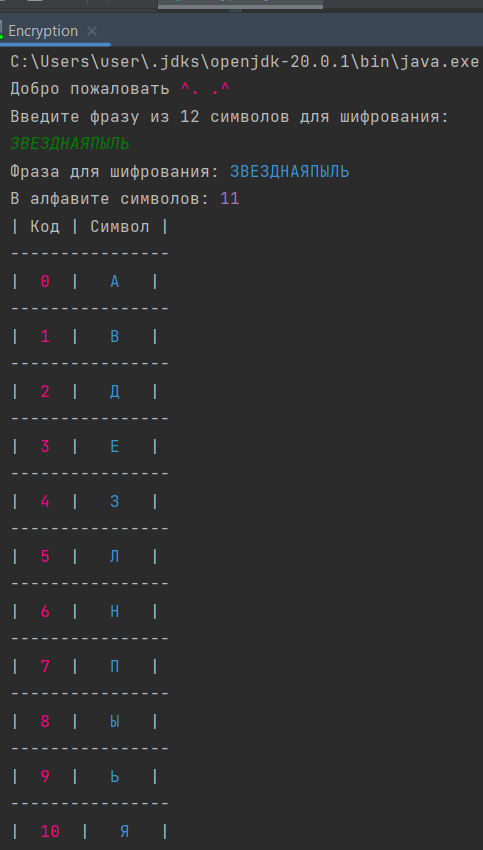
\includegraphics[width=1.25\linewidth]{лань1.png} \\ а)}
\end{minipage}
%\caption{Результат работы программы для ключа $2 \times 2$ .}
\label{ris:image1}
\end{figure}

\begin{figure}[h!]
\begin{minipage}[h!]{0.49\linewidth}
\center{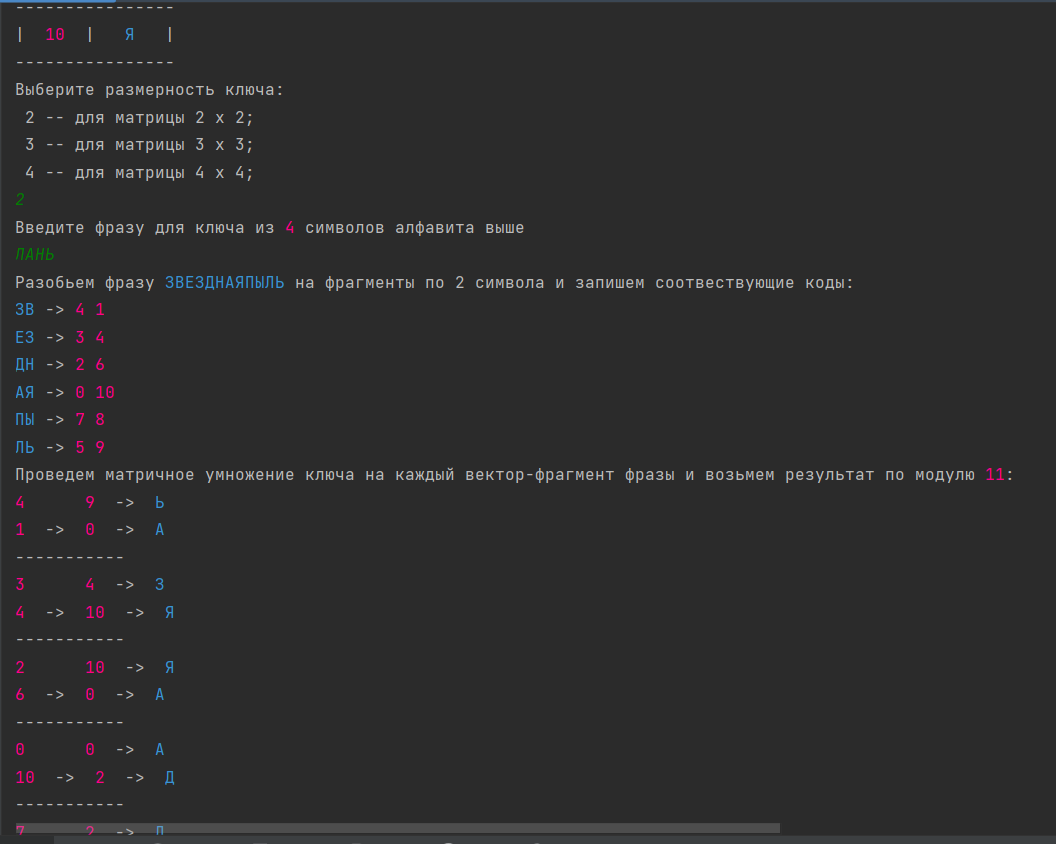
\includegraphics[width=2\linewidth]{лань2.png} \\ б)}
\end{minipage}
%\caption{Результат работы программы для ключа $2 \times 2$ .}
\label{ris:image1}
\end{figure}

\begin{figure}[h!]
\begin{minipage}[h!]{0.49\linewidth}
\center{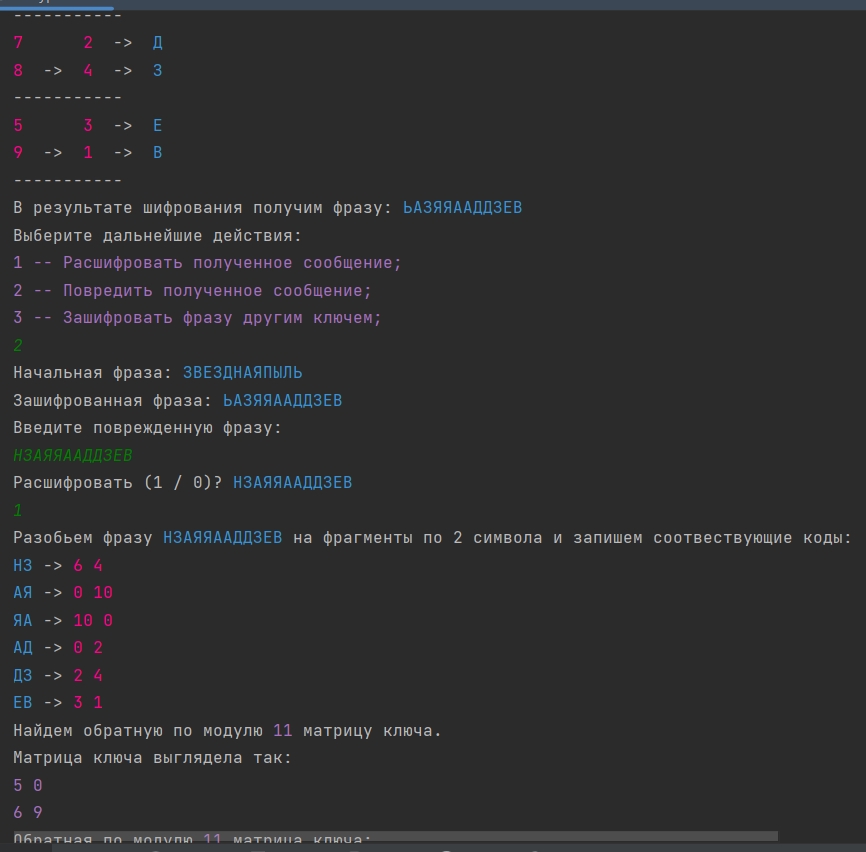
\includegraphics[width=2\linewidth]{лань3.png} \\ в)}
\end{minipage}
%\caption{Результат работы программы для ключа $2 \times 2$ .}
\label{ris:image1}
\end{figure}

\begin{figure}[h!]
\begin{minipage}[h!]{0.49\linewidth}
\center{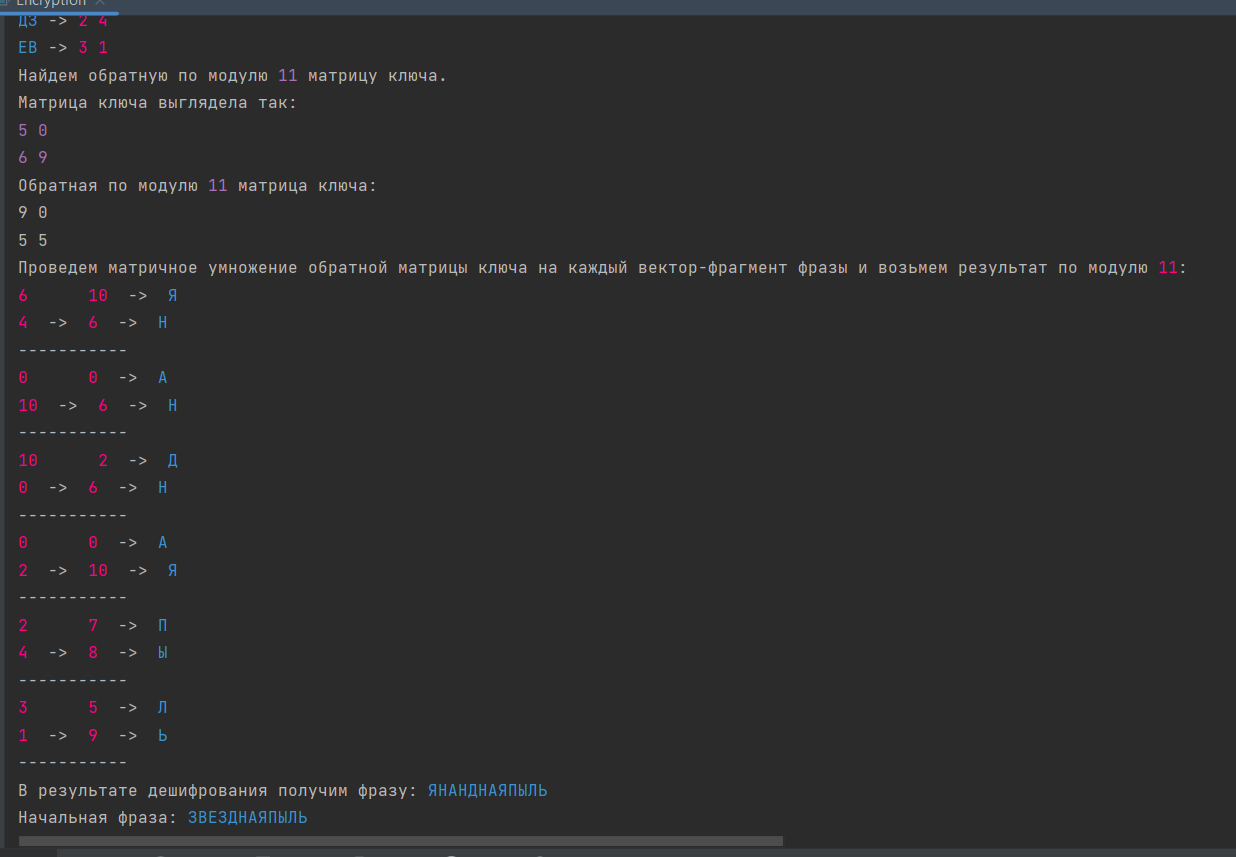
\includegraphics[width=2\linewidth]{лань4.png} \\ г)}
\end{minipage}
\caption{Результаты работы программы для ключа $2 \times 2$ .}
\label{ris:image1}
\end{figure}
\end{document}













